%%%%%%%%%%%%%%%%%%%%%%%%%%%%%%%%%%%%%%%%%%%%%%%%%%%%%%%%%%%%%%%%%%%%%%%%%%%%%%%%
%2345678901234567890123456789012345678901234567890123456789012345678901234567890
%        1         2         3         4         5         6         7         8

\documentclass[letterpaper, 10 pt, conference]{ieeeconf}  % Comment this line out if you need a4paper

%\documentclass[a4paper, 10pt, conference]{ieeeconf}      % Use this line for a4 paper

\IEEEoverridecommandlockouts                              % This command is only needed if 
                                                          % you want to use the \thanks command

\overrideIEEEmargins                                      % Needed to meet printer requirements.

% See the \addtolength command later in the file to balance the column lengths
% on the last page of the document

% The following packages can be found on http:\\www.ctan.org
\usepackage{graphics} % for pdf, bitmapped graphics files
\usepackage{epsfig} % for postscript graphics files
%\usepackage{mathptmx} % assumes new font selection scheme installed
\usepackage{times} % assumes new font selection scheme installed
\let\proof\relax
\let\endproof\relax
\usepackage{amsmath} % assumes amsmath package installed
\usepackage{amssymb}  % assumes amsmath package installed
\usepackage{amsthm}
\usepackage{algorithm}
\usepackage{algorithmicx}
\usepackage{algpseudocode}
\usepackage{xcolor}
\usepackage{subfigure}
\usepackage{multicol}

\newtheorem{proposition}{Proposition}
\newtheorem{remark}{Remark}
\title{\LARGE \bf
Smooth, Physically-Consistent Adaptive Control for Robot Manipulators
}


\author{Taeyoon Lee$^{1}$, Jaewoon Kwon$^{2}$ and Frank C. Park$^{3}$% <-this % stops a space
% \thanks{*This work was not supported by any organization}% <-this % stops a space
\thanks{$^{1}$Taeyoon Lee, $^{2}$Jaewoon Kwon and $^{3}$Frank Chongwoo Park  are with the Department of
Mechanical and Aerospace Engineering, Seoul National University, Seoul
08826, South Korea 
        {\tt\small fcp@snu.ac.kr}}%
}


\begin{document}



\maketitle
\thispagestyle{empty}
\pagestyle{empty}


%%%%%%%%%%%%%%%%%%%%%%%%%%%%%%%%%%%%%%%%%%%%%%%%%%%%%%%%%%%%%%%%%%%%%%%%%%%%%%%%
\begin{abstract}



\end{abstract}


%%%%%%%%%%%%%%%%%%%%%%%%%%%%%%%%%%%%%%%%%%%%%%%%%%%%%%%%%%%%%%%%%%%%%%%%%%%%%%%%
\section{INTRODUCTION}

The adaptive control, which has a technical goal of adapting the controller online even in the presence of model uncertainty, is an appealing strategy for taking account robustness for control in an intelligent manner. Adaptive control of robot manipulator, which is an appealing application for such method, has long been extensively studied throughout the past decades.

The two most important and globally convergent classes of adaptive controllers developed for robot manipulators are {\em adaptive inverse dynamics control}, or {\em adaptive computed torque control}, proposed by Craig et al \cite{Craig_AdaptiveControl}, and {\em passivity based adaptive control} proposed by Slotine and Li \cite{Slotine_AdaptiveControl}. The important distinction from the past works is that they are proven to be the globally convergent controller that does not rely on any linear approximation of the dynamic model, but utilizes the explicit linear decomposition of constant inertial parameters in the dynamics. 

One general assumption in {\em adaptive inverse dynamics control} \cite{Craig_AdaptiveControl} and other approaches[][] that fall into this category is the requirement of uniform positive definiteness of the estimated mass matrix, since the inverse of estimated mass matrix is explicitly used in the parameter adaptation law. Passivity based adaptive control \cite{Slotine_AdaptiveControl} enjoys some attractive advantages over adaptive inverse dynamics based approach, including the fact that uniform positive definiteness of the estimated mass matrix is not required for implementation of the algorithm. However, uniform positive definiteness of the estimated mass matrix may not end up to be simply a technical requirement for specific class of adaptive controller, but a desirable aspect for performance of general adaptive controller in a sense that the estimated parameters should guarantee to be a physically feasible one.

Positive definiteness requirement of the estimated mass matrix is directly related to the physical consistency of the estimated inertial parameters of a robot. It can be shown that the physical consistency condition on inertial parameters(i.e. positive mass and positive definite rotational inertial matrix at the center of mass) gurantee the positive definite requirement of the corresponding mass matrix. Exploiting this property together with convex characterization of the set of physically consistent inertial parameters, projection based algorithms or parameter resetting algorithms have been applied to robot adaptive control, which essentially switches the parameter update law on the boundary of feasible set to enforce the estimated parameter to be feasible, which in turn would produce a non-smooth adaptive controller when the parameter touches the user-specified boundary of feasible set.

In this paper, we propose a novel modification of parameter adaptation law that guarantees the physical consistency of estimated parameters in a smooth manner without having to explicitly specify feasible set of parameters and rely on projection or resetting based algorithms. Also, it does not require any additional computational supplement to the existing methods and is directly applicable to any globally convergent Lyapunov-based adaptive controllers that exploits the linear decomposition of inertial parameters in dynamics. Our adaptation law, which we would call {\em natural adaptation law}, also drastically reduces the requirement of engineering choice of adaptation gain matrix $\Gamma$. While the existing adaptation laws can be viewed as a gradient-like dynamics on flat Euclidean space with constant metric $\Gamma$, our method is a natural gradient-like dynamics on non-flat Riemannian space, where the natural Riemmanian metric defined on the space essentially determines the large portion of natural choice of adaptation gain matrix. With the requirement of small number of tunable parameter in the adaptive controller, our adaptive controller enjoys more ``intelligent" behavior of adaptation against the model uncertainty. Our method is validated via simulation experiment on 7-dof robot manipulator involving trajectory tracking tasks under uncertainty in entire set of inertial parameters of the manipulator, and subject to large unknown payload grasped by the end-effector. Also, adaptation of joint Coloumb friction parameters, having positive quantities in nature, is respected in a similar manner.

\section{Geometry of Rigid Body Inertial Parameter}
\subsection{Physically Consistent Rigid Body Inertial Parameters}
Inertial parameters that constitute the dynamics of a single rigid body include mass $m$, center of mass $p_{b}\in\mathbb{R}^{3}$ and symmetric $3\times 3$ matrix of rotational inertia tensor $I_{b}\in\mathcal{S}(3)$, all represented in body-fixed reference frame $\{b\}$. For the purpose of exploiting the linearity of inertial parameters in dynamic equations for various dynamics-based applications including dynamic identification and adaptive control, it is common to express them in the vectorized form,
\begin{equation*}
\phi_{b} = [m,h_{b},I_{b}^{xx},I_{b}^{yy},I_{b}^{zz},I_{b}^{xy},I_{b}^{yz},I_{b}^{zx}]\in\mathbb{R}^{10}
\end{equation*}
, where $h_{b} = mp_{b}\in \mathbb{R}^{3}$. It turns out that there are exactly ten number of independent variables for respresenting inertial parameters of a single rigid body. However, they are not valid over the whole $\mathbb{R}^{10}$ space but only the subset, since they are subject to so called physical consistency condition; there should exist at least a single nonnegative mass density function $\rho : \mathbb{R}^{3} \rightarrow \mathbb{R}^{+}_{0}$ that realizes the given the parameter $\phi_{b}$. As pointed out in \cite{Wittenberg_Dynamics}, \cite{Traversaro_IROS}, the requirement that a rigid body's mass $m$ be positive
and its inertia matrix at the center of mass, $I_{b}^{C}=I_{b}-m[p_{b}][p_{b}]^{T}$, be positive-definite is in fact a necessary, but not sufficient. So called triangular inequality condition on the three eigenvalues of $I_{b}^{C}$ has to hold additionally in order for the physically realizable nonnegative mass density function to exist. 

In \cite{Wensing_RAL} the equivalent full physical consistency condition is expressed in the following
alternative but equivalent form: the $4 \times 4$ symmetric matrix $P_{b} \in \mathcal{S}(4)$ 
is defined as 
\begin{eqnarray}
P_{b} = \int \left[\begin{array}{c} \vec{r}_{b} \\ 1 \end{array}\right]
  \left[\begin{array}{c} \vec{r}_{b} \\ 1 \end{array}\right]^{T} \rho(\vec{r}_b) dV_{b} 
= \left[\begin{array}{cc} \Sigma_{b} & h_{b} \\ h_{b}^{T} & m \end{array}\right],
\label{44psd}
\end{eqnarray}
where the second moment matrix $\Sigma_{b}\in \mathcal{S}(3)$ is defined by
$\Sigma_{b} = \int \vec{r}_{b}\vec{r}_{b}^{T} \rho(\vec{r}_{b})dV_{b}$.  It is shown
in \cite{Wensing_RAL} that the condition that $P_b$ be positive-definite, i.e.,
\begin{equation}
P_b \succ 0
\label{full_cond_44psd}
\end{equation}
is equivalent to the physical consistency conditions described in \cite{Traversaro_IROS}.
To make this identification more explicit, from the relation $\Sigma_{b}
= \frac{1}{2}\mathrm{tr}(I_{b})\mathbf{1} - I_{b}$, which holds for any choice of
body frame $\{b\}$, the one-to-one linear mapping $f : \mathbb{R}^{10}
\rightarrow \mathcal{S}(4)$ can be defined as follows:
\begin{align*}
&f(\phi_{b}) = P_{b} = \left[\begin{array}{cc} \frac{1}{2}\mathrm{tr}(I_{b})
\cdot\mathbf{1} - I_{b} & h_{b} \\ h_{b}^{T} & m\end{array}\right] \in \mathcal{S}(4)\\
&f^{-1}(P_{b}) = \phi_{b}(m, h_{b}, \mathrm{tr}(\Sigma_{b})\cdot\mathbf{1}
- \Sigma_{b}) \in \mathbb{R}^{10}.
\end{align*}
The physical consistency conditions on the  parameter $\phi_{b} \in \mathbb{R}^{10}$
can be identified under the mapping $f$ with the requirement that the symmetric matrix
$P_{b} = f(\phi_b) \in \mathcal{P}(4)$ be positive definite.

Based on the above, we define the manifold $\mathcal{M}$ of the set of physically consistent
inertial parameters for a single rigid body as follows:
\begin{align*}
\mathcal{M} &\simeq \{ \phi_{b} \in \mathbb{R}^{10} : f(\phi_{b}) \succ 0\}
\subset\mathbb{R}^{10}\nonumber\\
& \simeq \{ P_{b} \in \mathcal{S}(4) : P_{b} \succ 0\} = \mathcal{P}(4).
\end{align*}
The elements can be identified in both $\mathbb{R}^{10}$ and $\mathcal{P}(4)$, also
for different choices of body-fixed reference frame $\{b\}$. For a multibody system
with $n$ rigid links, the space of physically consistent inertial parameters is
given by the product space $\mathcal{M}^{n} \simeq \mathcal{P}(4)^{n}$.
\subsection{Riemannian Geometry of $\mathcal{M} \simeq \mathcal{P}(4)$ }
Riemmanian geometric structure can be defined on the manifold $\mathcal{M}$ with a natural choice of Riemmanian metric. In order for a distance to be naturally defined on a manifold, it is desirable to be invariant with respect to choice of coordinate frames or physical units/scale. It would also be desirable if the distance were to possess a physical meaning that corresponds to our intuition. The standard Euclidean metric on $\mathbb{R}^{10}$ under the vectorized representation $\phi_{b}$ is found to satisfy none of these desiderata \cite{Taeyoon_RAL}. Authors in \cite{Taeyoon_RAL} define a coordinate-invariant distance metric on $\mathcal{M}$ that is essentially inherited from the space of $\mathcal{P}(4)$ endowed with affine-invariant Riemannian metric; For $P \in \mathcal{P}(4)$ and tangent vector $X, Y \in T_{P}\mathcal{P}(4)$, Riemannian metric invariant under the group action $G * P = GPG^T$, where $G\in GL(4)$ is any $4\times 4$ non singular matrix, is given by
\begin{equation*}
\langle X,Y \rangle_{P} = \frac{1}{2}\mathrm{tr}(P^{-1}XP^{-1}Y).
\label{riem_metric_Pn}
\end{equation*}
Then the resulting geodesic distance between two arbitrary points $P_1, P_2 \in \mathcal{P}(4)$ is given by 
\begin{equation*}
d_{\mathcal{P}(4)}(P_1,P_2) = \bigg(\sum_{i=1}^{n}\big(\log(\lambda_{i})\big)^2\bigg)^{1/2},
\nonumber
\end{equation*}
where $\lambda_i$ are the eigenvalues of $P_{1}^{-1/2}P_{2}P_{1}^{-1/2}$,
or equivalently, those of $P_{1}^{-1}P_{2}$. Now, applying a one-to-one mapping $f$ from the vectorized inertial parameter $\phi_b$ to the matrix form $P_{b} = f(\phi_b)$, a distance metric on $\mathcal{M}$ is defined as,
\begin{equation}
d_{\mathcal{M}}({^{1}}\phi_{b}, {^{2}}\phi_{b})=d_{\mathcal{P}(4)}({^{1}}P_{b}, {^{2}}P_{b}),
\label{metric_singlebody}
\end{equation}
which was proven to be invariant to the choice of coordinate frames $\{b\}$ and physical unit/scale, and also possess some intersesting features that matches to our physical intuition and has close connection to the Fisher information metric as remarked in \cite{Taeyoon_RAL}.

\subsection{Bregman Divergence as a Pseudo Distance Metric on $\mathcal{M}$}
Riemmanian geometric approach in many engineering applications provides coordinate-invariant set of tools to treat data that can be sensitive to the coordinate choices. However, as will be specified in the following sections, exact Riemmanian geodesic distance defined as (\ref{metric_singlebody}) fails to be directly applicable to the existing framework of robot adaptive control for its algebraic nonlinearity.

In this section, we propose an alternative psuedo distance metric on inertial parameters that derives from the Bregman divergence of a log-det function on $\mathcal{P}(4)$, which still preserves coordinate-invariance property but is only non-negative and fails to be symmetric nor satisfy triangular inequality.

Bregman divergence associated with a function $F: \Omega\rightarrow \mathbb{R}$ for points $p,q\in\Omega$ is defined by the difference between the value of $F$ at point $p$ and the value of the first-order Taylor expansion of $F$ around point $q$ evaluated at point $p$:
\begin{equation*}
D_{F(\Omega)}(p || q) = F(p)-F(q)-\langle\nabla F(q), p-q\rangle.
\end{equation*}
When $\Omega = \mathcal{P}(4)$, the bregman divergence associated with a log-det function $F$, i.e. $F(P) = -\log|P|$ for $P\in\mathcal{P}(4)$, is given by,
\begin{align}
D_{F(\mathcal{P}(4))}(P || Q) &= \log\frac{|Q|}{|P|} + \mathrm{tr}(Q^{-1}P) - 4\\
&= \sum_{i=1}^4(-\log(\lambda_{i})+\lambda_{i}-1),
\end{align}
where $\lambda_i$ are the eigenvalues of $Q^{-1}P$ or equivalently $Q^{-1/2}PQ^{-1/2}$. Note that $D_{F(\mathcal{P}(4))}$ is affine-invariant, that is invariant under the $GL(4)$ group action $*$.

Again using the one-to-one mapping $f$ from $\phi$ to $P = f(\phi)$ we can define the distance measure on $\mathcal{M}$ as
\begin{equation}
D_{\mathcal{M}}({^{1}}\phi_{b}, {^{2}}\phi_{b}) = D_{F(\mathcal{P}(4))}({^{1}}P_{b} ||  {^{2}}P_{b}), \label{Bregman_div}
\end{equation}
which is coordinate-invaraint, since the coordinate transformation on $P$ follow the exact form of $GL(4)$ group action $*$ as described in \cite{Taeyoon_RAL}. We now omit all the coordinate frame subscripts for expressing the inertial paramters $\phi$ and $P$.
\begin{remark}
The divergence measure $D_{F(\mathcal{P}(n))}$ approximates affine-invariant Riemmanian metric up to second order; that is for two infinitesimally close positive definite matrices $P$ and $P +dP$, the following holds:
\begin{equation*}
D_{F(\mathcal{P}(n))}(P || P+dP) = \langle dP,dP \rangle_{P} + o(\lambda_i(P^{-1}dP)^3)
\end{equation*}
(((((Further relation to KL-divergence on Gaussian distributions)))))
\end{remark}

\subsection{Natural Gradient Descent on $\mathcal{M}$}
Natural gradient descent is a generalization of the steepest descent method on flat Euclidean space to a general curved Riemannian space \cite{Amari_Naturalgrad}. Let $g : \mathcal{P}(4) \rightarrow \mathbb{R}$ be a differentiable function defined on $\mathcal{M}$. Then the steepest descent direction of $g(P)$ at $P\in\mathcal{P}(4)$ is defined by the tangent vector $dP\in\mathcal{S}(4)$ that minimizes $g(P+dP) \simeq g(P) + \mathrm{tr}(\nabla g(P)\cdot dP)$ where $\|dP\|_{P}$ has a fixed length in terms of local Rimannian metric ($[\nabla g(P)]_{ij} \triangleq \partial g/\partial P_{ij}$). The ensuing optimization problem can be formulated as the following:
\begin{gather}
dP = \arg\min_{W} \mathrm{tr}(\nabla g(P)\cdot W) \\
 \text{s.t. } \|W\|_{P}^2= \frac{1}{2}\mathrm{tr}(P^{-1}WP^{-1}W) = 1 \label{norm_constraint}
\end{gather}
The Lagrangian for the above can be defined by $L(W, \lambda) = \mathrm{tr}(\nabla g(P)\cdot W) + \lambda(1- \mathrm{tr}(P^{-1}WP^{-1}W))$ and the first order necessary condition $\nabla_{W}L = 0$ yields the optimal $W$ as,
\begin{equation}
W = \gamma \cdot P\nabla g(P) P, \label{natural_gradient_direction}
\end{equation}
where the constant scalar $\gamma$ is determined from the constraint (\ref{norm_constraint}). Here, the natural gradient descent direction $P\nabla g(P) P$ clearly differs from the classical steepsest descent direction on Euclidean space, $\nabla g(P)$.
\section{Previous Results on Adaptive Control for Robot Manipulators}
Dynamic equations for general $n$-dof open chain manipulators take the form,
\begin{equation}
M(q,\Phi)\ddot{q}+C(q,\dot{q},\Phi)\dot{q} + g(q,\Phi) = u, \label{dynamics}
\end{equation}
where $q\in\mathbb{R}^n$ is the vector of joint angles, $M(\cdot)\in\mathbb{R}^{n\times n}$, $C(\cdot)\in\mathbb{R}^{n\times n}$, and $g(\cdot)\in\mathbb{R}^{n}$ denote the mass matrix, Coriolis matrix, and the gravitational force vector respectively, $u\in\mathbb{R}^{n}$ is the motor torque input, and $\Phi = [\phi_{1}^{T}, \cdots, \phi_{n}^{T}]^{T}\in\mathbb{R}^{10n}$ is the complete set of inertial parameters for $n$ links. The technical goal of adaptive and robust control is to design a control input $u$ that ensures global convergence of trajectory tracking error even in the presence of model uncertainty. In this paper, we confine our interest to the class of adaptive controllers that assumes only the model uncertainty in inertial parameter $\Phi$. Furthermore, as the term ``adaptive"  indicates, time-varying estimates of the true model parameters are respected together with the trajectory tracking controller, which differentiates from class of robust controllers that make use of fixed parameter estimates with known uncertainty bound.

Here we revisit the two important class of Lyapunov-based globally convergent adaptive controllers developed for robot manipulators in \cite{Craig_AdaptiveControl} and \cite{Slotine_AdaptiveControl}.
\subsection{Adaptive Computed Torque Control \cite{Craig_AdaptiveControl}}
The control input for Adaptive Computed Torque Control, also referred to as Adaptive Inverse Dynamics, is given by,
\begin{equation}
u = M(q,\hat{\Phi})\{\ddot{q}_{d}-K_{v}\dot{\tilde{q}}-K_{p}\tilde{q}\}+C(q,\dot{q},\hat{\Phi})\dot{q}+g(q,\hat{\Phi}), \label{ACTC_input}
\end{equation}
where $K_p\in\mathbb{R}^{n\times n}$ and $K_{v}\in\mathbb{R}^{n\times n}$ are diagonal matrices of positive gains, $q_{d}$ is the given reference trajectory, $\tilde{q} = q - q_d$, and $\hat{\Phi}$ is the estimate of the true inertial parameter $\Phi$, whose update law would be clarified later. Then using the linear property of inertial parameters in dynamic equations, the closed loop dynamics becomes
\begin{equation}
\ddot{\tilde{q}}+K_{v}\dot{\tilde{q}}+K_{p}\tilde{q}=M(q,\hat{\Phi})^{-1}Y(q,\dot{q},\ddot{q})\tilde{\Phi}, \label{ACTC_CL_dyn}
\end{equation}
where $Y\in \mathbb{R}^{n\times10n}$ is the regressor function that satisfies
\begin{equation}
M(q,\Phi)\ddot{q}+C(q,\dot{q},\Phi)\dot{q} + g(q,\Phi) = Y(q,\dot{q},\ddot{q})\Phi,
\end{equation}
 and $\tilde{\Phi} =\hat{\Phi}-\Phi$. The state space formulation of (\ref{ACTC_CL_dyn}) with augmented state vector defined as $e=[\tilde{q}^{T}, \dot{\tilde{q}}^{T}]^{T}$ is given by 
\begin{equation}
\dot{e} = Ae+BM(q,\hat{\Phi})^{-1}Y(q,\dot{q},\ddot{q})\tilde{\Phi}, \label{ACTC_CL_error_dyn}
\end{equation}
where $A = \left[\begin{array}{cc} 0 & I \\ -K_{p} & -K_{v}\end{array}\right]\in \mathbb{R}^{2n\times2n}$ is a Hurwitz matrix and $B=\left[\begin{array}{cc} 0 & I\end{array}\right]^T\in\mathbb{R}^{2n\times n}$. Then we may choose some $Q \in \mathcal{P}(n)$ and let $P \in \mathcal{P}(n)$ be the unique symmetric positive definite matrix satisfying the Lyapunov equation
\begin{equation}
A^{T}P + PA = -Q. \label{ACTC_lyapunov_eq}
\end{equation}
Now we define the Lyapunov function candidate $V$ as the following:
\begin{equation*}
V = e^{T}Pe + \tilde{\Phi}^{T}\Gamma\tilde{\Phi},
\end{equation*}
where $\Gamma$ is a constant symmetric positive definite matrix.
Then the time derivative of the Lyapunov function candidate $\dot{V}$ is derived from (\ref{ACTC_CL_error_dyn}) and (\ref{ACTC_lyapunov_eq}) as,
\begin{equation*}
\dot{V} = -e^{T}Qe + 2\tilde{\Phi}^{T}\{Y(q,\dot{q},\ddot{q})^{T}M(q,\hat{\Phi})^{-1}B^{T}Pe+\Gamma\dot{\hat{\Phi}}\},
\end{equation*}
also using the fact that $\dot{\tilde{\Phi}} = \dot{\hat{\Phi}}$, since $\Phi$ is constant. Choosing the parameter update law or adaptation law as,
\begin{equation}
\dot{\hat{\Phi}} = -\Gamma^{-1}Y(q,\dot{q},\ddot{q})^{T}M(q,\hat{\Phi})^{-1}B^{T}Pe, \label{ACTC_parameter_update}
\end{equation}
we have 
\begin{equation*}
\dot{V} = -e^{T}Qe \leq 0 .
\end{equation*}
From the stability analysis provided in \cite{Craig_AdaptiveControl} it follows that position tracking error $e$ converges to zero asymptotically and the parameter estimate error $\tilde{\Phi}^{T}\Gamma\tilde{\Phi}$ remains bounded, given that $M(q,\hat{\Phi})$ is bounded, and inverse of $M(q,\hat{\Phi})$ exists. Actually, $M(q,\hat{\Phi})$ must be invertible to implement the adaptation law (\ref{ACTC_parameter_update}) wherein the term $M(q, \hat{\Phi})^{-1}$ is explicitly used without justification of its existence. In \cite{Craig_AdaptiveControl}, authors provide ad-hoc strategy to reset or project the parameters to always reside inside some feasible bound defined by a set of linear inequality constraints on $\hat{\Phi}$ that sufficiently guarantees the boundedness and invertibility (or equivalently positive definiteness) of $M(q,\hat{\Phi})$. Another important issue in implementing the adaptation law (\ref{ACTC_parameter_update}) is the requirement of joint accelaration $\ddot{q}$ feedback, which is practically hard to measure or numerically differentiate from position or velocity with fine quality. The adaptive controller presented below proposed by Slotine and Li \cite{Slotine_AdaptiveControl} removes both of these impediments.
% However, the invertibility of estimated mass matrix is related to the physical consistency of inertial parameters and note that the Passivity-based Adaptive Control still do not guarantee the non-singularity or positive definiteness of $M(q,\hat{\Phi})$.
% \subsection{(Robust Adaptive Computed Torque Control)}
\subsection{Passivity-based Adaptive Control \cite{Slotine_AdaptiveControl}}
The control input for Passivity-based Adaptive Control is given by,
\begin{align}
u & = M(q,\hat{\Phi})a + C(q,\dot{q},\hat{\Phi})v + g(q,\hat{\Phi})-Kr, \label{PBAC_input}\\
& = Y(q,\dot{q}, a, v)\hat{\Phi} - Kr \nonumber
\end{align}
where the vectors $v,a,r\in\mathbb{R}^{n}$ are defined as
\begin{align*}
v = \dot{q}_{d}-\Lambda\tilde{q}, \quad
a = \dot{v} = \ddot{q}_{d}-\Lambda\dot{\tilde{q}}, \quad
r = \dot{q}-v = \dot{\tilde{q}}+\Lambda\tilde{q},
\end{align*}
and $K$ and $\Lambda$ are diagonal matrices of constant positive gains. Then the closed loop dynamics is given by,
\begin{equation*}
M(q,\Phi)\dot{r} + C(q,\dot{q},\Phi)r+Kr = Y(q,\dot{q},a,v)\tilde{\Phi}.
\end{equation*}
Here we introduce the Lyapunov function candidate as follows:
\begin{equation}
V = \frac{1}{2}r^{T}M(q,\Phi)r + \tilde{q}^{T}\Lambda K\tilde{q}+\frac{1}{2}\tilde{\Phi}^{T}\Gamma\tilde{\Phi} \label{Slotine_lyapunov}
\end{equation}
where $\Gamma$ is again set to be a constant symmetric positive definite matrix.
Using the skew-symmetry property of the matrix $\dot{M} - 2C$ \cite{Slotine_AdaptiveControl}, $\dot{V}$ is calculated as,
\begin{equation*}
\dot{V} = -\tilde{q}^{T}\Lambda K \Lambda\tilde{q} - \dot{\tilde{q}}^{T}K\dot{\tilde{q}} + \tilde{\Phi}^{T}\{\Gamma\dot{\hat{\Phi}} + Y^{T}r\}.
\end{equation*}
Choosing the parameter update law or adaptation law as,
\begin{equation}
\dot{\hat{\Phi}} = -\Gamma^{-1}Y(q,\dot{q},a,v)^{T}r, \label{PBAC_parameter_update}
\end{equation}
we have
\begin{equation*}
\dot{V} = -\left[\begin{array}{c} \tilde{q} \\ \dot{\tilde{q}}\end{array}\right]^{T}\left[\begin{array}{cc} \Lambda K \Lambda & 0 \\ 0 & K \end{array}\right]\left[\begin{array}{c} \tilde{q} \\ \dot{\tilde{q}}\end{array}\right] = -e^{T}Qe \leq 0.
\end{equation*}
It can also be shown that position tracking error $e$ converges to zero asymptotically and parameter estimate error remains bounded. Note that the acceleration measurements nor the inverse of $M(q,\hat{\Phi})$ is required for the control input and parameter update.

Natural and practical choice of gain matrix $K$ can be determined as, $K = \lambda\cdot M(q,\hat{\Phi})$ for some scalar constant $\lambda$ as noted in \cite{Slotine_Composite}, physically meaning that higher gain is used for joint with higher inertia. It is shown in \cite{Slotine_Composite} that despite of such time-varying choice of $K$ it guarantees the global convergence with a slight modification of $a$ in the regressor function $Y$ in adaptation law (\ref{PBAC_parameter_update}) to, $a-\lambda r$, and with $\Lambda = \lambda \cdot I$.

\section{Contribution: Natural Adaptaion Law}
Lyapunov stability analysis provides a technical way of assessing the stability of the closed loop system, where in the investigation of particular choice of Lyapunov function candidate is demanded. However, a natural choice of Lyapunov function candidate at firsthand can sometimes adversely help in designing the natural stabilizing control law. Especially for a large class of mechanical systems including robot manipulators, a branch of passivity-based control methods that exploits the skew-symmetry of $\dot{M} - 2C$ have been developed by considering the choice of energy-like Lyapunov function candidate, i.e. system's kinetic, elastic energy related functions as also in (\ref{Slotine_lyapunov}). Such method allows the closed loop system to inherit the intrinsic physical properties of the original system to some extent \cite{Slotine_Magazine}, rather than entirely substituting the original dynamics with that of virtual spring- damper system through feedback linearization as in computed-torque control. Slotine and Li, as described in the former section, has shown that such physically motivating control design can also be successfully applied to adaptive manipulator control.

Meanwhile, the general class of globally convergent adaptive control for robot manipulators discussed in the former section consider the Lyapunov function candidate $V$ as the summation of tracking error term $V_t$ and parameter error term $V_p$:
\begin{equation}
V = \underbrace{V_t(q,\dot{q},q_{d},\dot{q_{d}},\Phi)}_{\text{(tracking error)}} + \underbrace{V_p(\Phi, \hat{\Phi})}_{\text{(parameter error)}}.
\end{equation}
Here, as opposed to the choice of tracking error term $V_{t}$, the natural choice of parameter error term $V_{p}$ is often overlooked, in most cases naively considering quadratic parameter error of the from $\tilde{\Phi}^{T}\Gamma\tilde{\Phi}$ with constant positive definite matrix $\Gamma$. The effect of measuring the distance on vectorized representation of inertial parameters in such Euclidean sense has been discussed in \cite{Taeyoon_RAL}, highly susceptible to a fatal scale problem. This aspect easily leads to a physically inconsistent estimation of the parameters when measurement data is insufficient or excitation trajectory is non-persistent. Such problem should also be pervasive in adaptive control, wherein limited source of trajectory data is available for the parameters to be adapted online. For the case of adaptive computed-torque control where the invertibility of mass matrix $M(q,\hat{\Phi})$ is technically demanded, several projection or resetting based modification of the adaptation law has been proposed to keep estimated inertial parameters to be physically consistent \cite{Craig_AdaptiveControl}, \cite{Slotine_Indirect}, \cite{Ioannou_RAC}, \cite{Wang_Projection}, which sufficiently guarantees the uniform invertibility of $M(q,\hat{\Phi})$. However, such method is somehow an ad-hoc remedy to the problem which behaves conservative near the boundary of user-specified feasible region and can often produce non-smooth torque input. On the other hand, Slotine and Li have suggested indirect \cite{Slotine_Indirect} or composite version \cite{Slotine_Composite} of their passivity based method, where they take into account additional filtered torque prediction error in a least square sense which essentially updates the matrix $\Gamma$ to a more well-conditioned value over the time.

However, to the best of our knowledge, none of the adaptation laws so far respect the physical consistency of the estimated parameters in an intrinsic and smooth manner, which do not rely on any ad-hoc resetting or projection algorithm. In the following section, we argue that these desirable aspects can in fact be achieved by simply considering the natural and coordinate invariant choice of smooth parameter error term $V_{p}$ at firsthand, resulting in natural gradient-like adaptation law of the parameters.
\subsection{Bregman Divergence as a Lyapunov Function Candidate}
A seemingly possible and natural choice of $V_{p}$ could be a geodesic distance metric as defined in \cite{Taeyoon_RAL}, i.e. 
\begin{equation}
V_{p}(\Phi,\hat{\Phi}) = \sum_{i=1}^{n} d_{\mathcal{M}}(\phi_{i}, \hat{\phi_{i}}). \label{geodesic_distance}
\end{equation}
However, it turns out that such choice fails to argebraically enforce the negative-definiteness of $\dot{V}$ due to the nonlinearity of (\ref{geodesic_distance}). Recall that the time derivative of tracking error related Lyapunov function candidate $V_{t}$ is derived in the following form:
\begin{align}
\dot{V_t} &= -e^{T}Qe +\tilde{\Phi}^{T}b \label{dot_V_t}
% &= -e^{T}Qe + \tilde{\Phi}^{T}b + \tilde{\Phi}^{T}g(\dot{\hat{\Phi}}, \hat{\Phi})\nonumber\\
% &= -e^{T}Qe + \tilde{\Phi}^{T}\{b+ g(\dot{\hat{\Phi}}, \hat{\Phi})\nonumber\}
\end{align}
, where for the Adaptive Computed Torque Control $b = Y^T\hat{M}^{-1}B^{T}Pe$, and for the Passivity-based Adaptive Control $b = Y^{T}r$. In order to make the time derivative of the entire Lyapunov function candidate $V = V_{t}+V_{p}$ to be negative definite, time derivative of $V_{p}$ is algebraically required to be of the form,
\begin{equation}
\dot{V_{p}}(\Phi, \hat{\Phi})=\tilde{\Phi}^{T}g(\dot{\hat{\Phi}}, \hat{\Phi}) \label{dot_V_p},
\end{equation}
resulting in the adaptation law $g(\dot{\hat{\Phi}}, \hat{\Phi}) = - b$ and eventually $\dot{V} =\dot{V_{t}}+\dot{V_{p}}= -e^{T}Qe \leq 0$. When $V_{p}$ is set as conventional quadratic error, i.e. $V_{p} = \tilde{\Phi}^{T}\Gamma\tilde{\Phi}$, then $g(\dot{\hat{\Phi}}, \hat{\Phi}) = \Gamma \dot{\hat{\Phi}}$. Note here that $g$ should be a function of only estimated parameters $\hat{\Phi}$ and their time derivatives $\dot{\hat{\Phi}}$ and not include true parameter $\Phi$, since it is not known $a \ priori$, rather a desired value we wish to estimate. With the choice of $V_{p}$ in (\ref{geodesic_distance}), its time derivative fails to be explicitly factored in the form (\ref{dot_V_p}) at all for its nonlinearity.

We now claim that the Bregman divergence based distance measure discussed in (\ref{Bregman_div}) allows a valid Lyapunov function candidate of $V_{p}$ whose time derivative can actually be derived in the form (\ref{dot_V_p}).
\begin{proposition}
A function $V_{p}$ defined as
\begin{equation}
V_{p}(\Phi,\hat{\Phi}) = \gamma \sum_{i=1}^n D_{F(\mathcal{P}(4))}(f(\phi_{i}) || f(\hat{\phi_{i}})) \label{bregman_V_p}
%\left[\log\bigg(\frac{|f(\hat{\phi_{i}})|}{|f(\phi_{i})|}\bigg) + \mathrm{tr}(f(\hat{\phi_{i}})^{-1}f(\phi_{i})) - 4\right] 
\end{equation}
 for constant positive scalar gain $\gamma$ and true parameter vector $\Phi$ is a valid Lyapunov function candidate of $\hat{\Phi}$, which is differentiated in the form (\ref{dot_V_p}).

\begin{proof}
Firstly, it can be observed that $V_{p}$ is a symmetric function of a set of eigenvalues $\lambda_{i}^{j}$ ($j=1,2,3,4$) of matrices $f(\hat{\phi_{i}})^{-1}f(\phi_{i})$, which implies coordinate invariance of $V_{p}$. Explicitly $V_{p}$ is given by
\begin{equation*}
V_{p} = \gamma\sum_{i=1}^{n}\sum_{j=1}^{4}[ - \log(\lambda_{i}^{j}) + \lambda_{i}^{j} - 1].
\end{equation*}
Since a scalar function $-\log(x)+x-1$ is always non-negative, $V_{p}\geq 0$ is a valid Lyapunov function candidate, having zero only when $\lambda_{i}^{j} = 1$ for all $i,j$, i.e. $ \hat{\Phi} = \Phi$.

The time derivative of $V_{p}$ is given by,
\begin{align}
\dot{V_{p}} =&\gamma\frac{d}{dt}\sum_{i=1}^n\left[\log\bigg(\frac{|f(\hat{\phi_{i}})|}{|f(\phi_{i})|}\bigg) + \mathrm{tr}(f(\hat{\phi_{i}})^{-1}f(\phi_{i})) - 4\right] \nonumber\\
=&\gamma\sum_{i=1}^n \mathrm{tr}\bigg(f(\hat{\phi_{i}})^{-1}f(\dot{\hat{\phi_{i}}})-f(\hat{\phi_{i}})^{-1}f(\dot{\hat{\phi_{i}}})f(\hat{\phi_{i}})^{-1}f(\phi_{i})\bigg)\nonumber\\
=& \gamma\sum_{i=1}^n \mathrm{tr}\bigg(f(\hat{\phi_{i}})^{-1}f(\dot{\hat{\phi_{i}}})f(\hat{\phi_{i}})^{-1}(f(\hat{\phi_{i}})-f(\phi_{i}))\bigg)\nonumber\\
=&\gamma\sum_{i=1}^n \mathrm{tr}\bigg(\big[f(\hat{\phi_{i}})^{-1}f(\dot{\hat{\phi_{i}}})f(\hat{\phi_{i}})^{-1}\big]f(\tilde{\phi_{i}})\bigg)\label{dot_V_p_bregman}
\end{align}
, where we used the fact that $\frac{d}{dt}f(\hat{\phi})=f(\dot{\hat{\phi}})$ and $f(\hat{\phi})-f(\phi) = f(\hat{\phi}-\phi) = f(\tilde{\phi})$ which hold by the linearity of mapping $f$. Again by the linearity of $f$, $\dot{V_{p}}$ calculated above can be expressed in the form (\ref{dot_V_p}).
\end{proof}
\end{proposition}
\subsection{Natural Adaptation Law}
Based on the choice of $V_{p}$ as in (\ref{bregman_V_p}), we now propose a novel adaptation law applicable to any adaptive control methods in which the time derivative of tracking error related Lyapunov function candidate $V_{t}$ is expressible in the form (\ref{dot_V_t}).
\begin{proposition}
Given the control law that results in the time derivative of $V_{t}$ of the form (\ref{dot_V_t}), the following adaptation law:
\begin{equation}
\dot{\hat{P_i}} = -\frac{1}{\gamma}\hat{P_i} B_i \hat{P_i}, \qquad i = 1, \cdots, n \label{natural_adaptation_1}
\end{equation}
% or equivalently,
% \begin{equation}
% \frac{d}{dt}(\hat{P_i}^{-1}) = \frac{1}{\gamma}B_i, \qquad i = 1, \cdots, n \label{natural_adaptation_2}
% \end{equation}
, where $\hat{P_i} = f(\hat{\phi_i})$ and $B_i$ are unique symmetric matrices that satisfies the relation $\tilde{\Phi}^{T}b = \sum_{i=1}^n \mathrm{tr}(f(\tilde{\phi_i})B_i)$, gurantees the asymptotic convergence of tracking error to zero, bounded parameter error and also physical consistency of the estimated parameter $\hat{\Phi}$ over the time given that the initial estimate is chosen to be physically consistent.

\begin{proof}
Consider the valid Lyapunov function candidate,
\begin{equation*}
V = V_t + V_p
\end{equation*}
, where $V_p$ is defined by (\ref{bregman_V_p}). Then,
\begin{align*}
\dot{V} &= \dot{V_t} + \dot{V_p}\\
 &= -e^{T}Qe + \tilde{\Phi}^{T}b + \gamma\sum_{i=1}^n \mathrm{tr}\big(\hat{P_i}^{-1}\dot{\hat{P_i}}\hat{P_i}^{-1}\tilde{P_i}\big)\\
 &=-e^{T}Qe + \sum_{i=1}^n\mathrm{tr}(\tilde{P_i}B_i) + \gamma\sum_{i=1}^n \mathrm{tr}\big(\hat{P_i}^{-1}\dot{\hat{P_i}}\hat{P_i}^{-1}\tilde{P_i}\big)\\
 &= -e^{T}Qe + \sum_{i=1}^n \mathrm{tr}\big([B_i +\gamma\hat{P_i}^{-1}\dot{\hat{P_i}}\hat{P_i}^{-1}]\tilde{P_i}\big)
\end{align*}
holds from (\ref{dot_V_t}), (\ref{dot_V_p_bregman}) and $\tilde{P_i} = f(\tilde{\phi_i}) = \hat{P_i}-P_i$. From the adaptation rule defined by (\ref{natural_adaptation_1}),
\begin{equation*}
\dot{V} = -e^{T}Qe \leq 0
\end{equation*}
holds and the asymptotic convergence of tracking error can be shown in the same manner as before. Moreover, since $\dot{V} \leq 0$, $V$ is bounded and therefore $V_p = V - V_t \leq V$ is always bounded over the time. Meanwhile, $V_p(0)$ is truly bounded, since initial parameter estimate is set to be physically consistent, i.e. $\hat{P_i}(0) \in \mathcal{P}(4)$. If there exists some time instance $T>0$ where $\hat{P_i}(T)$ is not positive definite, then by the continuity there exists time instance $0<t_0\leq T$ such that $\hat{P_i}(t_0)$ is on the boundary of $\mathcal{P}(4)$, i.e. at least one of the eigenvalues of $\hat{P_i}(t_0)$ is zero. Then this contradicts the fact that $V_p(t)$ be bounded for all $t>0$, since $V_p(t_0)$ is infinity. Therefore, the present adaptation law always gurantees the physical consistency of $\hat{\Phi} \sim \{\hat{P_i}\}_{i=1}^n$.
\end{proof}
\end{proposition}
% \begin{remark}
As was shown, the adaptation law (\ref{natural_adaptation_1}) theoretically assures the physical consistency of the estimated parameters; that is $\hat{P_i}$ are always updated to be positive definite regardless of $\gamma$ and $B_{i}$. However, from the view of practical implementatin of the adaptation law, when preset gain $1/\gamma$ or $B_{i}$ in some time instance is large relative to the discrete time step size, the naive Euler integration on Euclidean space as,
\begin{equation*}
\hat{P_i}(t+\Delta t) = \hat{P_i}(t) - \frac{1}{\gamma}\hat{P_i}(t)B_{i}(t)\hat{P_i}(t)\cdot\Delta t
\end{equation*}
or from equivalent expression of (\ref{natural_adaptation_1}) as $\frac{d}{dt}(\hat{P_i}^{-1}) = \frac{1}{\gamma}B_i$,
\begin{equation*}
\hat{P_i}(t+\Delta t) = (\hat{P_i}(t)^{-1} + \frac{1}{\gamma}B_{i}(t)\cdot\Delta t)^{-1}
\end{equation*}
, might not gurantee the positive definiteness of $\hat{P}_i$ over the time, although the continuous version of the algorithm guarantees such aspect. Therefore, we recommend to update $\hat{P}_i$ by exponential map or geodesic path on $\mathcal{M} \simeq \mathcal{P}(4)$ as,
\begin{align}
\hat{P_i}(t+\Delta t) &= \mathrm{Exp}_{\hat{P_i}(t)}\bigg(-\frac{1}{\gamma}\hat{P_i}(t)B_{i}(t)\hat{P_i}(t)\cdot\Delta t\bigg) \nonumber\\
&=\hat{P_i}(t)^{1/2}e^{-\frac{\Delta t}{\gamma}\hat{P_i}(t)^{1/2}B_i(t)\hat{P_i}(t)^{1/2}}\hat{P_i}(t)^{1/2} \label{natural_adaptation_discrete}
\end{align}
, which always gurantees the positive definiteness of $\hat{P}_i$. One might try to update (\ref{ACTC_parameter_update}) or (\ref{PBAC_parameter_update}) also with exponential map on the chance of guranteeing the physical consistency of estimated parameters. However, this would rather deter the stability of the system behaviour, since the update rule in (\ref{ACTC_parameter_update}) or (\ref{PBAC_parameter_update}) usually do require estimation of parameters to be physically inconsistent during the adaptation.

From the optimization perspective, the existing parameter update rules (\ref{ACTC_parameter_update}), (\ref{PBAC_parameter_update}) can be understood as steepest gradient descent-like method on the flat Euclidean space. The resetting or projection based modification of the existing methods is essentially stopping the update instantaneously or enforcing the descent direction to the feasible region when the parameter is about to cross the boundary of the feasible region. On the other hand, our method is analogous to the natural gradient descent method that generalizes the steepest descent method to the general non-flat Riemannian manifold. ((natural gradient provide more efficient direction of descent, which intrinsically enjoys no adaptaion dead zone.)) Note also that the exact Riemannian metric was not used to derive the adaptation law at firsthand, but the resulting natural gradient-like modification, i.e. from $\dot{P}_i \sim -B_i$ (which is equivalent to $\dot{\Phi} \sim b$) to $ \dot{P}_i\sim -P_iB_iP_i$, actually turn out to be the exact form of natural gradient (\ref{natural_gradient_direction}) on $\mathcal{P}(4)^n$ whose stabilizing property was instead proven from the use of Bregman divergence under Lyapunov-based analysis. 

Engineering choice of $\Sigma$... in [performance in adaptive control] least square based gain matrix used. which essentially needs prior trajectory... Our method only reduces to determine single parameter.. adaptation speed.. more intelligent! in a sense that human enigneering choice is minimized
% \end{remark}
% \begin{remark}
% Physical dimension analysis
% \end{remark}
% \begin{remark}
% Natural gradient $\nabla^2 F = G$, $[\nabla^2 F]^{-1}\frac{\partial f}{\partial x}$
% \end{remark}
% \begin{remark}
% Passivity preserving integrator of $\tilde{\Phi}$ to $b$ [Applied Nonlinear Control, page. 421]
% \end{remark}
% \begin{remark}
% Extension to composite adaptive control
% \end{remark}
%\section{Recursive Dynamics for torque input}


\begin{multicols}{1}
\begin{figure*}[!htb]
\centering
\begin{subfigure}
\centering
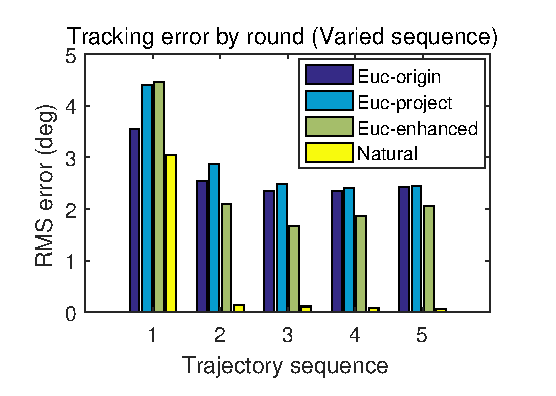
\includegraphics[width=.5\textwidth]{fig/ByRoundVaried.eps}
\caption{Tracking error of the varied sequence}
\label{fig:varied}
\end{subfigure}
\begin{subfigure}
\centering
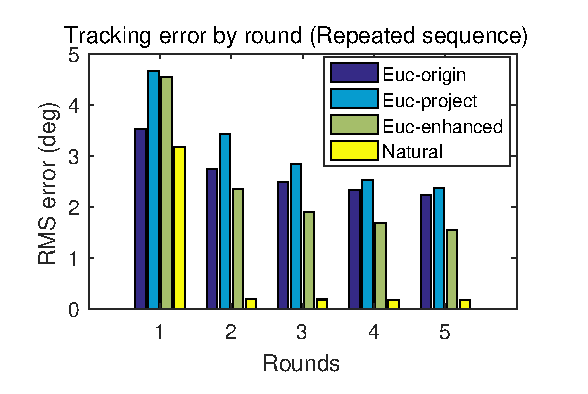
\includegraphics[width=.5\textwidth]{fig/ByRoundRepeated.eps}
\caption{Tracking error of the repeated sequence}
\label{fig:repeated}
\end{subfigure}
\end{figure*}
\end{multicols}

\section{Simulation Results}
The simulations are conducted in MATLAB and the manipulator we used is Barett WAM 7-DOFs manipulator arm model. The manipulator is assumed to be equipped with a torque-controller and fixed on the ground base. Self-collision and frictions are not considered yet. In order to make the simulation environment realistic and practical as possible, the control frequency is set as 1 kHz and the payload is limited to 3 kg. Although it is a tempting option to use {\it{ode45}} function of MATLAB for dynamic simulation, a simple Euler method is adopted since the adaptation of the inertial parameter will be updated digitally in real implementation.

The common task of all experiments is to track a joint space trajectory sequence which is composed of five unit trajectories. Each unit trajectory has a period of 5 seconds. Two types of sequences are used, which we refer to as a repeated sequence and a varied sequence. The repeated sequence is constructed from five identical cosine curves and the varied sequence is also constructed from the cosine curves but different amplitudes evenly spaced from $0.4$ to $1.2$. The unit trajectory is synthesized as follows:
\begin{equation*}
	q_i(t) = A_i~(\cos(\frac{2\pi}{T_i}t)-1)  \quad (i=1,\cdots,n)
\end{equation*}
where $q_i$ is the joint angle of the $i$th joint, $A_i$ is the amplitude,  $T_i$ is the period and $i$ is the joint number. There are four acronyms to indicate different adaptive control algorithms to be compared: 'Euc-origin' method is the original passivity-based adaptive control described in Section \ref{section2}. 'Euc-project' method is the modified method which projects the inertia tensors to satisfy physically-consistency and 'Euc-enhanced' method is another 'Euc-enhanced' method that uses constant pullback metric on initial estimate; $\Gamma$ is determined properly by the nominal parameters of the inertias. Finally, 'Natural' method indicates our proposed adaptive control algorithm. 

The same control gains are used for each experiment:  $\Lambda = 30.0\cdot I, ~\Gamma^{-1} = 0.0001\cdot I$ and $\gamma^{-1} = 1.0$. It might be noticed that the scale of $\Gamma$ and $\gamma$ is quite different, but those are not comparable by simply subtracting each other. The body links of the manipulator are visualized as ellipsoids which are physically-equivalent. That is, the inertia tensor of an ellipsoid is identical to that of the corresponding link. 

In Section \ref{section:entire}, it is assumed that nominal inertial parameters are given and the adaptations are applied to the entire set of the robot body. In Section \ref{section:EFonly}, three unknown loads are subjected to be adapted while the true parameters of the robot body inertias are known.


\subsection{Adaptation of Entire Set of Inertial Parameters} \label{section:entire}
In this section, an adaptation of the whole body is discussed. For the first experiment, the desired trajectory is a repeated sequence with a constant amplitude of 0.8. The nominal parameter is slightly perturbed from the true parameters as follows: $I_i \leftarrow k I_i + \frac{2}{5}m_{\text{perturb}}R_{\text{perturb}}^2$, $[h_i]\leftarrow k [h_i] $ and $m_i \leftarrow k ~m_i + m_{\text{perturb}}$, where $I_i$, $h_i$ and $m_i$ are inertial moment, center of mass and mass of the $i$th link, respectively. The perturbation $m_{\text{perturb}}=1.0$kg, $R_{\text{perturb}}=0.1$m and $k=0.9$. 

For the second experiment, the desired trajectory is the varied sequence composed of five unit trajectories, whose amplitudes are 1.2, 1.0, 0.8, 0.6 and 0.4. By changing the trajectories, the generalizability can be revealed from this experiment. It is said to be 'generalizable' when an adapted parameter by a certain training set also works well in an arbitrary test set. If an adaptive control shows poor generalizability, then it could behave unsafely or unexpectedly while tracking a new trajectory. The Figure~\ref{fig:varied}



\subsection{Adaptation of Unknown Load} \label{section:EFonly}
Repeated trajectory

As previously mentioned, the transient tracking error is not converged in any case by 'Euc-origin' method while 'Euc-enhnaced' method converged except the asymmetric load of the third case and 'Natural' is converged in all cases. 

Note that the RMS tracking error of the third load is initially the lowest by 'Euc-origin' method.

% \subsection{Selecting a Template (Heading 2)}

% First, confirm that you have the correct template for your paper size. This template has been tailored for output on the US-letter paper size. 
% It may be used for A4 paper size if the paper size setting is suitably modified.

% \subsection{Maintaining the Integrity of the Specifications}

% The template is used to format your paper and style the text. All margins, column widths, line spaces, and text fonts are prescribed; please do not alter them. You may note peculiarities. For example, the head margin in this template measures proportionately more than is customary. This measurement and others are deliberate, using specifications that anticipate your paper as one part of the entire proceedings, and not as an independent document. Please do not revise any of the current designations

% \section{MATH}

% Before you begin to format your paper, first write and save the content as a separate text file. Keep your text and graphic files separate until after the text has been formatted and styled. Do not use hard tabs, and limit use of hard returns to only one return at the end of a paragraph. Do not add any kind of pagination anywhere in the paper. Do not number text heads-the template will do that for you.

% Finally, complete content and organizational editing before formatting. Please take note of the following items when proofreading spelling and grammar:

% \subsection{Abbreviations and Acronyms} Define abbreviations and acronyms the first time they are used in the text, even after they have been defined in the abstract. Abbreviations such as IEEE, SI, MKS, CGS, sc, dc, and rms do not have to be defined. Do not use abbreviations in the title or heads unless they are unavoidable.

% \subsection{Units}

% \begin{itemize}

% \item Use either SI (MKS) or CGS as primary units. (SI units are encouraged.) English units may be used as secondary units (in parentheses). An exception would be the use of English units as identifiers in trade, such as Ò3.5-inch disk driveÓ.
% \item Avoid combining SI and CGS units, such as current in amperes and magnetic field in oersteds. This often leads to confusion because equations do not balance dimensionally. If you must use mixed units, clearly state the units for each quantity that you use in an equation.
% \item Do not mix complete spellings and abbreviations of units: ÒWb/m2Ó or Òwebers per square meterÓ, not Òwebers/m2Ó.  Spell out units when they appear in text: Ò. . . a few henriesÓ, not Ò. . . a few HÓ.
% \item Use a zero before decimal points: Ò0.25Ó, not Ò.25Ó. Use Òcm3Ó, not ÒccÓ. (bullet list)

% \end{itemize}


% \subsection{Equations}

% The equations are an exception to the prescribed specifications of this template. You will need to determine whether or not your equation should be typed using either the Times New Roman or the Symbol font (please no other font). To create multileveled equations, it may be necessary to treat the equation as a graphic and insert it into the text after your paper is styled. Number equations consecutively. Equation numbers, within parentheses, are to position flush right, as in (1), using a right tab stop. To make your equations more compact, you may use the solidus ( / ), the exp function, or appropriate exponents. Italicize Roman symbols for quantities and variables, but not Greek symbols. Use a long dash rather than a hyphen for a minus sign. Punctuate equations with commas or periods when they are part of a sentence, as in

% $$
% \alpha + \beta = \chi \eqno{(1)}
% $$

% Note that the equation is centered using a center tab stop. Be sure that the symbols in your equation have been defined before or immediately following the equation. Use Ò(1)Ó, not ÒEq. (1)Ó or Òequation (1)Ó, except at the beginning of a sentence: ÒEquation (1) is . . .Ó

% \subsection{Some Common Mistakes}
% \begin{itemize}


% \item The word ÒdataÓ is plural, not singular.
% \item The subscript for the permeability of vacuum ?0, and other common scientific constants, is zero with subscript formatting, not a lowercase letter ÒoÓ.
% \item In American English, commas, semi-/colons, periods, question and exclamation marks are located within quotation marks only when a complete thought or name is cited, such as a title or full quotation. When quotation marks are used, instead of a bold or italic typeface, to highlight a word or phrase, punctuation should appear outside of the quotation marks. A parenthetical phrase or statement at the end of a sentence is punctuated outside of the closing parenthesis (like this). (A parenthetical sentence is punctuated within the parentheses.)
% \item A graph within a graph is an ÒinsetÓ, not an ÒinsertÓ. The word alternatively is preferred to the word ÒalternatelyÓ (unless you really mean something that alternates).
% \item Do not use the word ÒessentiallyÓ to mean ÒapproximatelyÓ or ÒeffectivelyÓ.
% \item In your paper title, if the words Òthat usesÓ can accurately replace the word ÒusingÓ, capitalize the ÒuÓ; if not, keep using lower-cased.
% \item Be aware of the different meanings of the homophones ÒaffectÓ and ÒeffectÓ, ÒcomplementÓ and ÒcomplimentÓ, ÒdiscreetÓ and ÒdiscreteÓ, ÒprincipalÓ and ÒprincipleÓ.
% \item Do not confuse ÒimplyÓ and ÒinferÓ.
% \item The prefix ÒnonÓ is not a word; it should be joined to the word it modifies, usually without a hyphen.
% \item There is no period after the ÒetÓ in the Latin abbreviation Òet al.Ó.
% \item The abbreviation Òi.e.Ó means Òthat isÓ, and the abbreviation Òe.g.Ó means Òfor exampleÓ.

% \end{itemize}


% \section{USING THE TEMPLATE}

% Use this sample document as your LaTeX source file to create your document. Save this file as {\bf root.tex}. You have to make sure to use the cls file that came with this distribution. If you use a different style file, you cannot expect to get required margins. Note also that when you are creating your out PDF file, the source file is only part of the equation. {\it Your \TeX\ $\rightarrow$ PDF filter determines the output file size. Even if you make all the specifications to output a letter file in the source - if your filter is set to produce A4, you will only get A4 output. }

% It is impossible to account for all possible situation, one would encounter using \TeX. If you are using multiple \TeX\ files you must make sure that the ``MAIN`` source file is called root.tex - this is particularly important if your conference is using PaperPlaza's built in \TeX\ to PDF conversion tool.

% \subsection{Headings, etc}

% Text heads organize the topics on a relational, hierarchical basis. For example, the paper title is the primary text head because all subsequent material relates and elaborates on this one topic. If there are two or more sub-topics, the next level head (uppercase Roman numerals) should be used and, conversely, if there are not at least two sub-topics, then no subheads should be introduced. Styles named ÒHeading 1Ó, ÒHeading 2Ó, ÒHeading 3Ó, and ÒHeading 4Ó are prescribed.

% \subsection{Figures and Tables}

% Positioning Figures and Tables: Place figures and tables at the top and bottom of columns. Avoid placing them in the middle of columns. Large figures and tables may span across both columns. Figure captions should be below the figures; table heads should appear above the tables. Insert figures and tables after they are cited in the text. Use the abbreviation ÒFig. 1Ó, even at the beginning of a sentence.

% \begin{table}[h]
% \caption{An Example of a Table}
% \label{table_example}
% \begin{center}
% \begin{tabular}{|c||c|}
% \hline
% One & Two\\
% \hline
% Three & Four\\
% \hline
% \end{tabular}
% \end{center}
% \end{table}


%    \begin{figure}[thpb]
%       \centering
%       \framebox{\parbox{3in}{We suggest that you use a text box to insert a graphic (which is ideally a 300 dpi TIFF or EPS file, with all fonts embedded) because, in an document, this method is somewhat more stable than directly inserting a picture.
% }}
%       %\includegraphics[scale=1.0]{figurefile}
%       \caption{Inductance of oscillation winding on amorphous
%        magnetic core versus DC bias magnetic field}
%       \label{figurelabel}
%    \end{figure}
   

% Figure Labels: Use 8 point Times New Roman for Figure labels. Use words rather than symbols or abbreviations when writing Figure axis labels to avoid confusing the reader. As an example, write the quantity ÒMagnetizationÓ, or ÒMagnetization, MÓ, not just ÒMÓ. If including units in the label, present them within parentheses. Do not label axes only with units. In the example, write ÒMagnetization (A/m)Ó or ÒMagnetization {A[m(1)]}Ó, not just ÒA/mÓ. Do not label axes with a ratio of quantities and units. For example, write ÒTemperature (K)Ó, not ÒTemperature/K.Ó

\section{CONCLUSIONS}

% \addtolength{\textheight}{-0cm}   % This command serves to balance the column lengths
                                  % on the last page of the document manually. It shortens
                                  % the textheight of the last page by a suitable amount.
                                  % This command does not take effect until the next page
                                  % so it should come on the page before the last. Make
                                  % sure that you do not shorten the textheight too much.

%%%%%%%%%%%%%%%%%%%%%%%%%%%%%%%%%%%%%%%%%%%%%%%%%%%%%%%%%%%%%%%%%%%%%%%%%%%%%%%%



%%%%%%%%%%%%%%%%%%%%%%%%%%%%%%%%%%%%%%%%%%%%%%%%%%%%%%%%%%%%%%%%%%%%%%%%%%%%%%%%



%%%%%%%%%%%%%%%%%%%%%%%%%%%%%%%%%%%%%%%%%%%%%%%%%%%%%%%%%%%%%%%%%%%%%%%%%%%%%%%%
\section*{APPENDIX}

Appendixes should appear before the acknowledgment.

\section*{ACKNOWLEDGMENT}

% The preferred spelling of the word ÒacknowledgmentÓ in America is without an ÒeÓ after the ÒgÓ. Avoid the stilted expression, ÒOne of us (R. B. G.) thanks . . .Ó  Instead, try ÒR. B. G. thanksÓ. Put sponsor acknowledgments in the unnumbered footnote on the first page.


\begin{thebibliography}{99}
\bibitem{Wittenberg_Dynamics}  J. Wittenburg, {\em Dynamics of multibody systems}, Springer Science \& Business Media, 2007.
\bibitem{Traversaro_IROS} S. Traversaro, S. Brossette, A. Escande and F. Nori, ``Identification of fully physical consistent inertial parameters using optimization on manifolds", {\em 2016 IEEE/RSJ International Conference on Intelligent Robots and Systems (IROS)}, pp. 5446-5451, 2016.
\bibitem{Wensing_RAL} P. M. Wensing, S. Kim and J. J. E. Slotine, ``Linear matrix inequalities for physically consistent inertial parameter identification: a statistical perspective on the mass distribution", {\em IEEE Robotics and Automation Letters}, vol. 3, no. 1, pp. 60-67, Jan. 2018.
\bibitem{Taeyoon_RAL} T. Lee and F. C. Park, ``A geometric algorithm for robust multibody inertial parameter identification'', {\em IEEE Robotics and Automation Letters}, To appear
\bibitem{Amari_Naturalgrad} S. Amari, ``Natural Gradient Works Efficiently in Learning", {\em Neural Computation}, vol. 10, no. 2, pp. 251-276, Feb. 1998.
\bibitem{Craig_AdaptiveControl} J. J. Craig, P. Hsu and S. S. Sastry, ``Adaptive control of mechanical manipulators", {\em The International Journal of Robotics Research}, vol. 6, issue. 2, pp. 16-28, 1987.
\bibitem{Slotine_AdaptiveControl} J. J. E. Slotine and W. Li, ``On the adaptive control of robot manipulators", {\em The International Journal of Robotics Research}, vol. 6, issue. 3, pp. 49-59, 1987. 
\bibitem{Slotine_Magazine} J. J. E. Slotine, ``Putting physics in control-the example of robotics", {\em IEEE Control Systems Magazine}, vol. 8, no. 6, pp. 12-18, Dec. 1988.
\bibitem{Slotine_Indirect} W. Li and J. J. E. Slotine, ``Indirect adaptive robot control", {\em  1988 IEEE International Conference on Robotics and Automation}, vol. 2, pp. 704-709, 1988.
\bibitem{Slotine_Composite} J. J. E. Slotine and W. Li, ``Composite adaptive control of robot manipulators", {\em Automatica}, vol. 25, no. 4, pp. 509-519, 1989.
\bibitem{Ioannou_RAC} P. A. Ioannou and J. Sun, {\em Robust adaptive control}, Prentice Hall, 1996
\bibitem{Wang_Projection} H. Wang and Y. Xie, ``On the uniform positive definiteness of the estimated inertia for robot manipulators", {\em IFAC Proceedings Volumes }, vol. 44, issue. 1, pp. 4089-4094, 2011.


\end{thebibliography}




\end{document}
